% !TEX root = mythesis.tex

%==============================================================================
\chapter{Detector Exposure and Limits to the Diffuse Flux of UHE\texorpdfstring{$\nu$}{}s}
\label{chap:exp_limits_diffuse}
%==============================================================================
 
This chapter aims to detail the procedure used to calculate the detector exposure or sensitivity to neutrinos for the DG$\mathrm{_{\text{low}}}$ region. The efficiencies calculated in the last chapter are used and the final expected neutrino rates are calculated. The first part of the chapter describes the exposure calculation along with the exposure contribution from different channels. Systematic uncertainties which can arise during the full analysis along with their contribution to the exposure are also discussed. 
The second part of the chapter details the results of the unblinding where no possible neutrino candidates were found for the investigated angular range. Using this information an upper limit on the incoming flux of UHE$\nu$s is calculated. This limit is further compared to the one obtained by the previous analysis for the same time period but without the contribution of new triggers. The overall improvement to this limit is a crucial result of this work. 


\section{Exposure Calculation}
\label{sec:det_exposure_calc}

Exposure refers to the effective observation capability of a detector or observational setup over a specific time period, accounting for its sensitivity, the area it covers, and the duration of the observation. One of the most accurate techniques used at Auger to calculate the exposure of the SD array to UHE$\nu$s is through extensive simulations of different detector configurations. In this method MC neutrino showers are thrown over varied detector configuration to calculate the effective or active area at each instant of time. Since the detector configuration of the SD array is constantly changing (\textit{faulty tanks, regular maintenance etc.}), sometimes on a daily basis, this technique requires a large amount of computational time and resources making it less desirable for use in this analysis. 

\begin{figure}[t!]
  \centering
  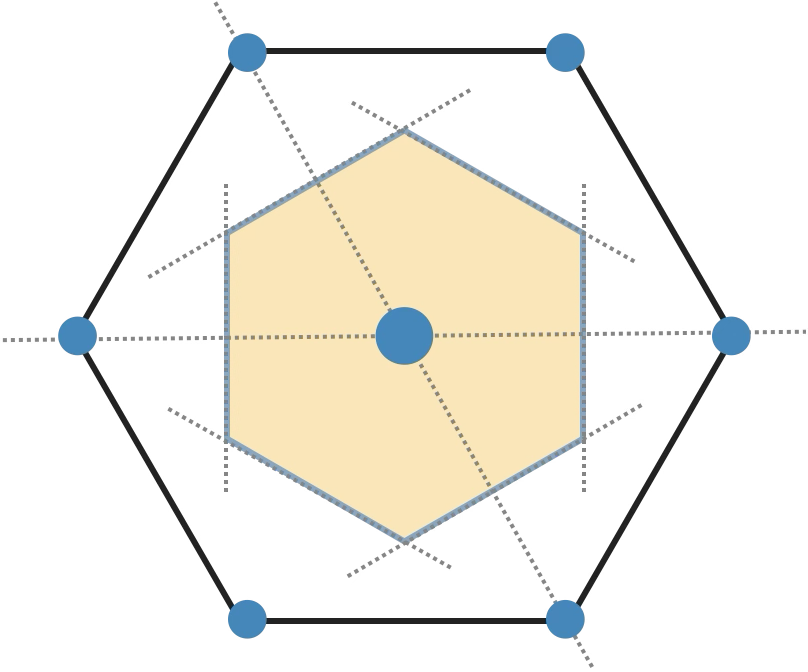
\includegraphics[width=0.5\textwidth]{thesis_figures/ExpLimits/Brillouin_area.png}
  \caption{Sketch of a 6T5 hexagon of the SD array. The shaded area in yellow represents the Brillouin effective area ($A_{6T5}$) of the hexagon for a neutrino event.}
  \label{fig:Brillouin_area}
\end{figure}

A different approach based on the 6T5 condition, which is required for each selected event for this study, is used for the exposure calculation. For this calculation, the 6T5 hexagon is taken to be the smallest possible detection unit for the $\nu$ event. The effective area i.e. the area where the neutrino can be observed for this detection unit at full efficiency is given by the Brillouin area~\cite{PierreAuger:2010zof}, $A_{6T5} = 1.95\,\mathrm{km}^2$ as shown by the shaded area in Fig.~\ref{fig:Brillouin_area}. The aperture for this detector unit is dependent on the energy of the primary neutrino, the slant depth in the atmosphere of the first interaction, X, neutrino flavor (cross-section), type of the interaction (CC or NC), zenith angle, azimuth angle and the point of impact of the shower on the ground. The effective \textit{acceptance} of the detector unit can be written as follows:

\begin{equation}
  \label{eq:nu_accep}
  A_{hex}(E_{\nu}, X)  = \int^{\phi = 2\pi}_{\phi = 0} \,d\phi \int_{\theta_{min} = 58.5^{\circ}}^{\theta_{max}= 76.5^{\circ}}  \, A_{6T5} \cdot \varepsilon(E_{\nu}, X, \theta) \cdot \sin \theta \, \cos \theta \cdot d\theta, \quad   \mathrm{[cm^2 sr]}
\end{equation}

where $\varepsilon(E_{\nu}, X, \theta)$ is the neutrino detection efficiency for each simulated energy, slant depth and zenith angle discussed in the last chapter. An example for a particular combination is given in Fig.~\ref{fig:Eff_X_comp} in the last chapter. Plots for efficiency for each combination can be found as part of the git repository made available for this analysis.

The next step involves integrating the \textit{acceptance} over the different simulated injected slant depths (as given in Tab.~\ref{tab:Simulation_params}) to account for the \textit{effective mass} target for the neutrino identification over the 6T5 hexagon unit. It is calculated as follows: 

\begin{equation}
  \label{eq:nu_eff_mass}
  M_{\text{hex}}(E_{\nu}) = \int_X A_{\text{hex}}(E_{\nu}, X) \cdot dX.
\end{equation}

Fig.~\ref{fig:EffMass_flavors_comp} shows the effective mass for both CC and NC interaction channels for a single 6T5 hexagon unit. Like the detection efficiency it increases with energy. 

\begin{figure}[t!]
  \centering
  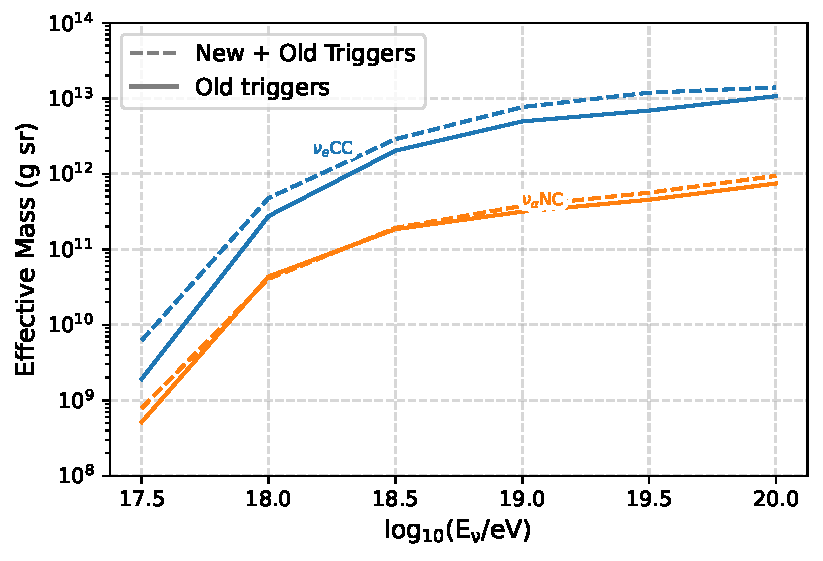
\includegraphics[width=14.5cm]{thesis_figures/ExpLimits/EffMass_comp_all_new_sim_optim.pdf}
  \caption{Effective mass for one 6T5 hexagon of the SD array for different neutrino flavors and interaction channels. The dashed lines are the calculated effective mass for this analysis and the solid lines is the effective mass calculated for the analysis performed without including new triggers.}
  \label{fig:EffMass_flavors_comp}
\end{figure}
Exposure calculation still needs to account for the detector configuration and its evolution over time. We reduced our array to units of 6T5 hexagons and a full SD array with 1660 stations consists 1420 of these hexagons. Since the establishment of the Pierre Auger Observatory the active number of 6T5 hexagons are monitored every second. This forms a very good indicator for the time evolution of the SD array since any non-working station or large periods of instability are intrinsically recorded in the number of active 6T5 hexagons at that time. The instantaneous number of hexagons, $n_{\text{hex}}(t)$ thus can be used as an indicator of detector configurations over time. The $n_{\text{hex}}(t)$ were updated and calculated every minute and have an uncertainty of about 1.5\% as mentioned in~\cite{PierreAuger:2010zof} and also confirmed in this study. To calculate the energy dependent exposure, the effective mass of one 6T5 hexagon is multiplied by the instantaneous number of hexagons and integrated in time. Further, the $\nu$ interaction probability for each flavour (i = $\nu_e, \nu_{\mu}, \nu_{\tau}$) and channel (c = CC, NC) is also folded in. The exposure is given as:

\begin{equation}
  \xi^{i,c}(E_{\nu}) = \frac{\sigma^{i,c}(E_{\nu})}{m_N} \int_{t} M_{\text{hex}}^{i,c}(E_{\nu}) \cdot n_{\text{hex}}(t) \cdot dt =  \frac{\sigma^{i,c}(E_{\nu})}{m_N} \cdot M_{\text{hex}}^{i,c}(E_{\nu}) \cdot N_{\text{hex}},
\end{equation}

$\sigma^{i,c}(E_{\nu})$ is the neutrino nucleon cross-section taken from~\cite{Cooper-Sarkar:2011jtt} and $N_{hex}$ is the total number of active 6T5 hexagons integrated in time over the search period. The value for $N_{hex}$ calculated for the period analysed is 2.8 $\times 10^{11}$ which is about $\sim$6.75 equivalent years of a fully functional SD array. The energy dependent exposure for different flavors and interaction channels is shown in Fig.~\ref{fig:Exp_flavors_comp}. It is necessary to point out again that the double bang showers which can be produced by $\nu_{tau}$ are not taken into account for this analysis.

\begin{figure}[t!]
  \centering
  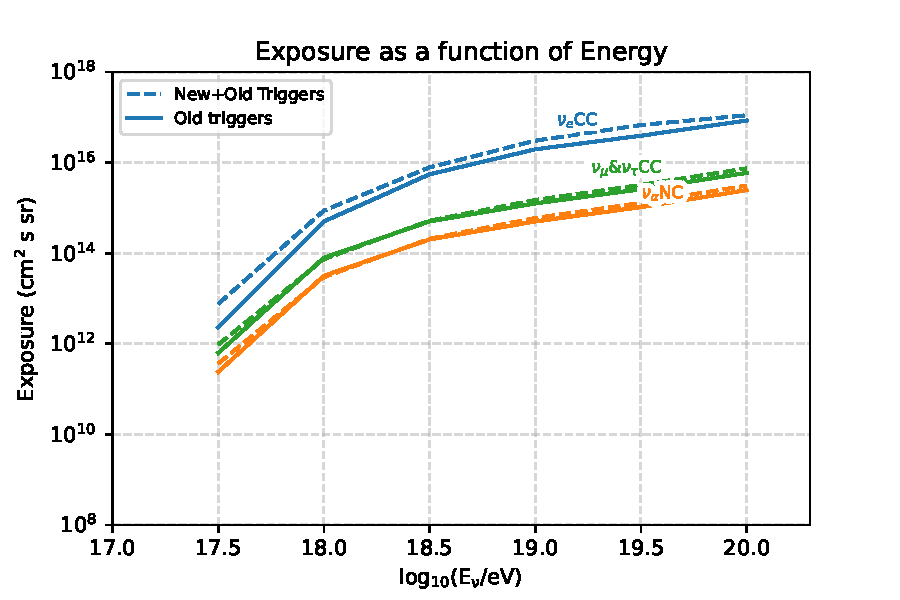
\includegraphics[width=14.5cm]{thesis_figures/ExpLimits/Exposure_comp_all_anotated_new_sim_optim.pdf}
  \caption{Exposure of the Pierre Auger Observatory for different neutrino flavors and interaction channels in the DG$_{\text{\text{low}}}$ angular range for the time period 2014-2021. The dashed lines are the calculated exposures for this analysis and the solid lines is the exposure calculated for the analysis performed without including new triggers for the same time period.}
  \label{fig:Exp_flavors_comp}
\end{figure}

An effective or total exposure, $\xi_{tot}(E_{\nu}) = \sum_{i}\sum_{c} \xi^{i,c}(E_{\nu})$ is calculated by summing all the interaction channels and assuming a 1:1:1 flavour ration at earth (large propagation distances combined with neutrino oscillations) as shown by the red line in Fig.~\ref{fig:Exp_total_comp}. 

\begin{figure}[t!]
  \centering
  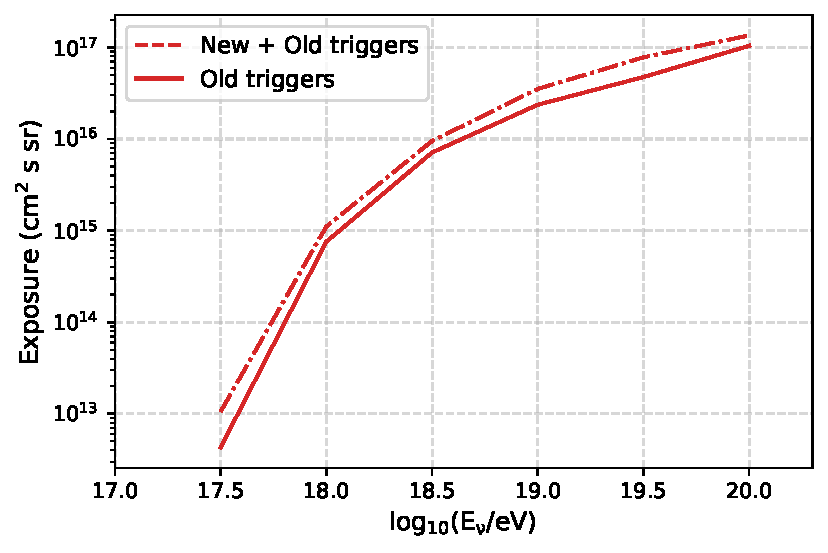
\includegraphics[width=14.5cm]{thesis_figures/ExpLimits/Exposure_comp_total_new_sim_optim.pdf}
  \caption{Comparison of the total exposure of the Pierre Auger Observatory for the time period 2014-2021. The dashed dotted line is the exposure calculated for this analysis and the solid line is the exposure calculated for the analysis performed without including new triggers for the same time period.}
  \label{fig:Exp_total_comp}
\end{figure}

As seen in the figure, the $\nu_e$ CC channels contributes the most to the total neutrino exposure ($\sim$85\%). The exposure rises rapidly at lower energies and then mostly flattens with just a slight increase which is due to the energy dependence of the neutrino cross-section. The shape is due to the neutrino detection efficiency which is small for lower energies as shown in Fig.~\ref{fig:Eff_v_theta_CC_E} in the previous chapter. The next dominant channels are the $\nu_{\tau}$ and $\nu_{\mu}$ CC which are assumed to have a similar detection efficiency as the NC channel but have a higher value of cross-section. The NC channel contribution is not significant ($\sim$5\%) due to the reasons discussed in section~\ref{subsec:nu_sel_nudeteff}.  

The exposure calculated in this analysis is also compared to the one calculated using the previous analysis for the same time period in Fig.~\ref{fig:Exp_flavors_comp}. For the CC channel a $\sim 5 \times$ improvement is seen at lower energies and a $\sim 2\times$ improvement at higher energies. For NC this improvement is not that significant. There is a $2\times$ improvement at lower energies and a 1.5$\times$ improvement at higher energies. The improvement at lower energies is due to the inclusion of the new triggers MoPS and ToTd which enhance the detection efficiency at lower energies. The improvement at higher energies is mainly due to the improved Fisher analysis. Since the $\nu_e$ CC contribution to the total exposure is significantly higher than other channels, the overall improvement to the total exposure is only slightly less than the improvement to the $\nu_e$ CC channel. 

\section{Systematic uncertainties}
\label{sec:det_uncert}
This section aims to detail the systematic uncertainties which can arise during the course analysis and their contribution to the exposure. The systematic uncertainties in an analysis can arise at any point. The investigations start already at the simulation level where the uncertainties from the primary interaction, hadronic interaction models, thinning etc. can lead to uncertainties in the neutrino detection efficiency. At the next step the uncertainties in the reconstruction algorithms could also affect the final exposure. The cross-sections used for the final calculation of exposure could also prove to be a source of systematic uncertainties. Other parameters such as the number of hexagons are very well-defined parameters and are not expected to have a contribution to the systematic uncertainties in the exposure. For this analysis the systematic uncertainties are either sourced through previous analysis~\cite{gap_systematics} or are calculated for certain cases. Since the analysis has been done once before, albeit without the new triggers, the sources of systematic uncertainties are sufficiently similar to~\cite{gap_note_2013}. 
The sources of systematic uncertainties considered for this analysis are discussed below:
\begin{description}
  \item \textbf{Primary interaction generator:} For the simulations used in this analysis which is based on CORSIKA 7.2 the only available option for the primary interaction generator is the HERWIG~\cite{Corcella:2000bw} code. Thus, it was not possible to compare the differences that could arise due to the use of different primary interaction generators. These systematic uncertainties were taken from ~\cite{gap_systematics} where PYTHIA~\cite{Sjostrand:2006za} and several versions of HERWIG are compared for CORSIKA 6. The uncertainties were found to be [+2.6\%, 3.7\%]. 
  \item \textbf{Parton Distribution function:} Again the uncertainties are taken from~\cite{gap_systematics} since this functionality is not available in CORSIKA 7. The systematic uncertainties on exposure quoted by the source are [+4\%, -5\%].
  \item \textbf{Hadronic interaction models:} The choice of the hadronic model used for the simulations can also lead to systematic uncertainties since most of these models are tuned on different accelerator datasets measured at much lower energies than the ones investigated in this analysis. Since the systematic uncertaintes due to the hadronic models calculated in this analysis were found to be below the statistic uncertainties. A realistic estimate of the systematic uncertainties due to the hadronic models was taken from~\cite{gap_systematics}, particularly the uncertainty between QGSJET-II and SIBYLL which is the closest analogy to this study where SIBYLL 2.3d was chosen as the reference model. The systematic uncertainties were chosen to be $+ 1\%$.
  \item \textbf{Shower simulator and thinning algorithm:} The systematic uncertainties due to the differing shower simulation programs was estimated through the comparison quoted in~\cite{Huege:2022xbo} for both hadronic cascades and electromagnetic showers. The differences seen in different softwares are of the order $\sim 15\%$ which agrees with the results from~\cite{gap_systematics}. The uncertainties due to thinning were also calculated in~\cite{gap_systematics} and were found to be $\sim 7\%$.
  \item \textbf{Detector simulation:} The differences in the detector simulation software i.e. a GEANT4 based approach used in this analysis to other approaches is already compared in~\cite{gap_note_det_systematics}. The systematic uncertainties were found to be $\pm 5\%$. Further, in this analysis the simulated showers were reconstructed using two different Offline tags with no significant differences observed in the final exposure. 
  \item \textbf{Number of Hexagons:} To calculate the total numbers of hexagons it is implicitly assumed that all stations contribute equally. However, if the new triggers are not active due to problems with two PMTs in a given station, such a hexagon might not contribute the same as the other. This points to a systematic error associated with using the hexagon files as they are, as a station with one PMT is counted full but likely should not. For a neutrino analysis with new triggers, the unique situation of an active WCD station which is unable to use these triggers needs to be accounted for. The systematic uncertainty associated with this effect was calculated by looking at the average number of stations with only one functional PMT over time. The uncertainty associated with this effect was found to be $\leq \pm 2\%$.
  \item \textbf{Reconstruction algorithm:} The effect of different reconstruction algorithm were also tested in this analysis. Two modules HASReconstructionOG and the normal top-down selection module were tested. Though the total number of events that are reconstructed by these modules can differ the difference in the final exposure is found to be $< \pm 1\%$. 
  \item \textbf{Neutrino cross-sections:} The systematic uncertainties due to the neutrino cross-sections were taken from~\cite{Cooper-Sarkar:2011jtt} which are of the order $\pm 7\%$.
\end{description}

Table~\ref{tab:systematic_uncertainties} summarizes the  source of systematic uncertainties and their contribution to the total exposure. The total systematic uncertainties are calculated by adding them in quadrature. As discussed later in section~\ref{subsec:Conrad} the uncertainties are directly incorporated in the limit by applying the Conrad method~\cite{Conrad:2002kn} to calculate the confidence intervals. 

\begin{table}[h!]
  \centering
  \begin{tabular}{ |P{6.0cm}||P{4.0cm}| }
    \hline
    Source of systematic uncertainty & Contribution \\
    \hline
    Primary interaction generator & +3\% \enspace -4\%  \\
    Parton Distribution function & +4\% \enspace -5\%  \\
    Hadronic interaction models & +1\% \\ 
    Shower simulator &  +15\%  \\
    Thinning algorithm & +7\% \enspace -7\%  \\
    Detector simulation & +5\% \enspace -5\%  \\
    Number of Hexagons & +2\% \enspace -2\%  \\
    Reconstruction algorithm & +1\% \enspace -1\%  \\
    Neutrino cross-sections & +7\% \enspace -7\%  \\
    \hline
    Total uncertainty & +19.5\% \enspace -13\% \\
    \hline
  \end{tabular}
  \caption{Systematic uncertainties and their contribution to the exposure}
  \label{tab:systematic_uncertainties}
\end{table}

\begin{figure}[ht!]
  \centering
  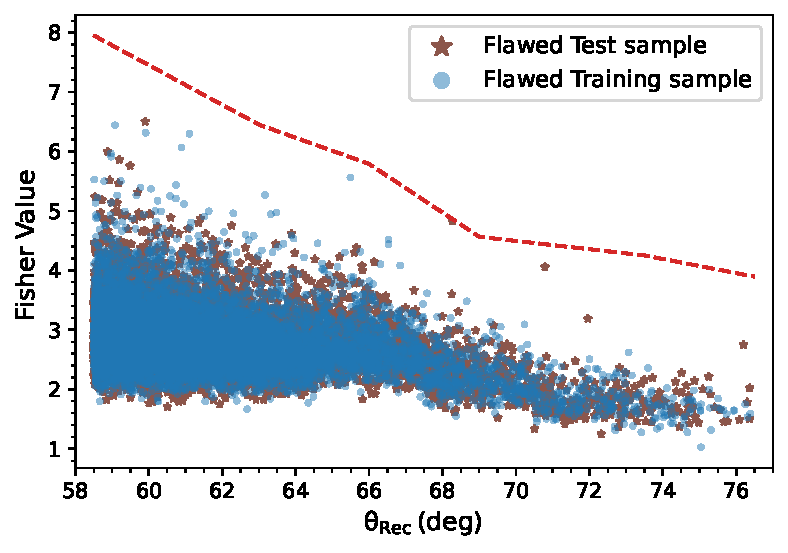
\includegraphics[width=0.95\textwidth]{thesis_figures/Nu_analysis/Fisher_plots/Fisher_comp_bkg_test_flawed_wnt.pdf}
  \caption{Distribution of the Fisher values for the background training sample (blue) and the test sample (brown) as a function of $\theta_{\text{Rec}}$ for the sample before the last fixes to the reconstruction were applied. The red line represents the interpolated $\mathcal{F}_{cut}$. The interesting events are marked with circles.}
  \label{fig:Fish_bkg_test_flawed}
\end{figure}

\section{Data unblinding}
\label{sec:data_unblinding}
As mentioned before in section~\ref{subsec:nu_sel_samp} the search data consists of all events recorded at the Observatory between 2014-2021 which have a SD ID number non-divisible by 5 i.e. 80\% of all SD data recorded between 2014-2021. This search data sample was further split into a 20\% test sample such that from the 80\% sample only those events where SD ID numbers were divisible by 4 were taken to be a part of the test sample while the rest became the part of the 60\% search sample. This split was done to perform the unblinding in two stages. The first, where only the test sample in unblinded to detect any remaining flaws in the analysis. This exercise turned out to be useful as a slight error was uncovered during the unblinding process of the 20\% test sample and was corrected. Said flaw, which is described in more detail later, required the whole reconstruction process along with the training of the Fisher polynomial to be performed again. This also effectively led to the unblinded 20\% test sample to be re-blinded since the reconstruction was altered. The splitting procedure was repeated and the total unblinding was performed again in parts. It is important to mention in all of unblinding procedure \textbf{0 neutrino events survive} the analysis selection.
This section is thus split into two subsections. The first describing the unblinding of the 20\% test sample along with the changes brought about by this unblinding. The second section details the full unblinding of the redone search samples (test + remaining) and discusses the interesting features of the unblinded search samples. 

\begin{table}[t!]
  \centering
  \begin{tabular}{ |P{3.0cm}||P{2.0cm}||P{4.0cm}| }
    \hline
    SD Event ID & $\theta_{\text{Rec}}$ & Reason \\
    \hline
    32988124 & $71.96^{\circ}$ & MoPS peak selection  \\
    40284452 & $58.88^{\circ}$ & No particular feature  \\
    45782830 & $65.50^{\circ}$ & No particular feature  \\
    54246856 & $70.79^{\circ}$ & MoPS Peak selection  \\
    66106356 & $68.30^{\circ}$ & Accidental station cut  \\
    \hline
  \end{tabular}
  \caption{Summary of the vents analysed in more detail from the flawed 20\% test sample. Some of these events are also discussed in App.~\ref{sec:app_3}.}
  \label{tab:Interesting_events}
\end{table}

\subsection{Flawed 20\% test sample}
\label{subsec:unblind_20}

The Fisher value distribution for the test sample is shown in Fig.~\ref{fig:Fish_bkg_test_flawed} where it is clear that no event passes the Fisher cut in any angular region. However, there are a few events which come very close to the cut line. Five events marked with a red circle were analysed in more detail. Each of them has its own unique reason with the one with zenith angle of $68.30^{\circ}$ and SD Event ID of "66106356" being the most interesting. After investigating the event in detail it was found that the accidental station cut used is insufficient. Previously, the  accidental cut (rejection of stations with Total signal < 3 VEM) is only applied to the event if there are more than 5 stations in the event. Since for this analysis due to the inclusion of MoPS and ToTd an overall increase in events is expected, which also increases the overall number of stations with accidental stations, this cut needs to be reduced a bit to take this overall increase into account. Thus, this cut was reduced to apply for events with more than 4 stations. This reduction of the cut decreases the total events passing the analysis cut by $\sim$5\% for the background training sample and $1-2$\% for the signal training sample. The Fisher coefficients and cuts change slightly. After this change in the reconstruction the test sample was obtained again and compared to the background sample as shown in Fig.~\ref{fig:Fish_bkg_test}. The other interesting events which have $\mathcal{F}$ values close to the $\mathcal{F}_{\text{cut}}$ with their respective IDs are tabulated in Tab.~\ref{tab:Interesting_events}. These events were individually evaluated. Some of these were found to have a bad time residual fit primarily because of multiple peaks observed in stations triggered by the new triggers. Since no segmentation algorithm was used for stations with MoPS and ToTd triggers, sometimes a wrong peak was selected, affecting the reconstruction for these events. A future analysis with a corrected segmentation algorithm which is functional for the new triggers MoPS and ToTd is envisaged as the next step. Such events are expected to be limited to less than $\sim$1\% of total events but still require a careful look for future analysis upgrades. A further detailed analysis where the primary mass composition is extracted via the muon production distributions, as mentioned in~\cite{PierreAuger:2014zay}, could not be performed for these events since the event had too few stations ($\sim 4$) and the shower had a very low reconstructed energy both of which hinder the ability to extract any information about the primary. Such events were also seen in previous analysis albeit not these many. For the other events no particular feature worth mentioning was observed. Some figures with more information about the interesting events from this section are also included as a part of App.~\ref{sec:app_3}. 



\begin{figure}[t!]
  \centering
  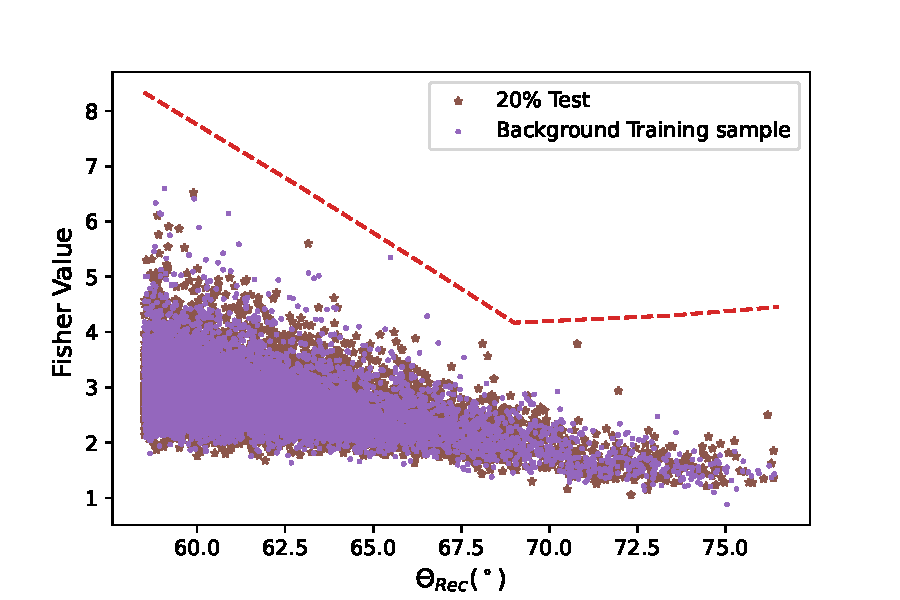
\includegraphics[width=0.95\textwidth]{thesis_figures/Nu_analysis/Fisher_plots/Fisher_comp_bkg_test_wnt.pdf}
  \caption{Distribution of the Fisher values for the background training sample (purple) and the test sample (brown) as a function of $\theta_{\text{Rec}}$. The red line represents the interpolated $\mathcal{F}_{\text{cut}}$.}
  \label{fig:Fish_bkg_test}
\end{figure}

\begin{figure}[t!]
  \centering
  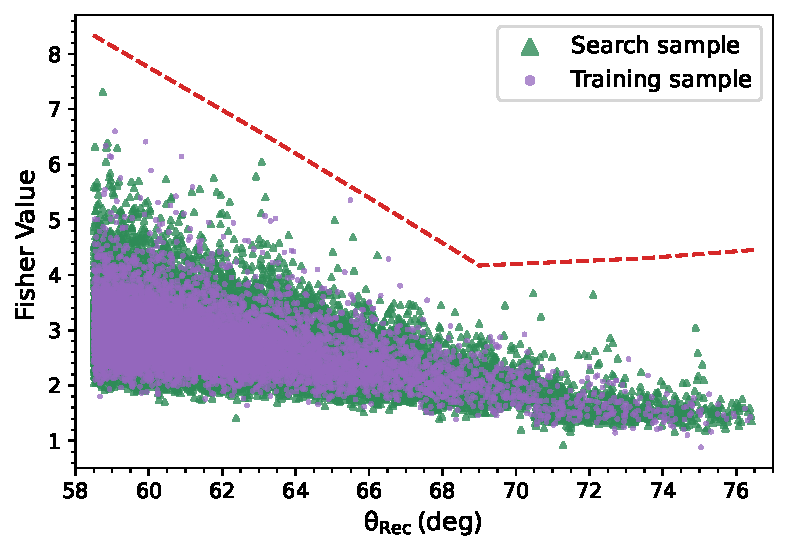
\includegraphics[width=0.95\textwidth]{thesis_figures/Nu_analysis/Fisher_plots/Fisher_comp_bkg_search_wnt.pdf}
  \caption{Distribution of the Fisher values for the background training sample (purple) and the search sample (green) as a function of $\theta_{\text{Rec}}$. The red line represents the interpolated $\mathcal{F}_{\text{cut}}$.}
  \label{fig:Fish_bkg_search}
\end{figure}

\subsection{Reevaluated 20\% test search sample and 60\% search sample}
\label{subsec:unblind_60}
After the errors discovered in the initial partial unblinding were fixed by altering the reconstruction, the final unblinding was again performed in two stages. Initially a 20\% part was unblinded and then the remaining 60\% blinded sample was analysed. Again \textbf{0 neutrino candidates} were found after candidate selection. The Fisher value distributions as a function of reconstructed zenith angle for both the test and search samples are presented in Fig.~\ref{fig:Fish_bkg_test} and Fig.~\ref{fig:Fish_bkg_search} respectively. The results of the test sample (brown) and search sample (green) are overlaid over the background training sample (purple) in each plot with the dashed lines indicating the value of the $\mathcal{F}_{\text{cut}}$ obtained according to eq.~\ref{eq:fisher_poly_cut}. As it can be seen the distributions are compatible with each other within statistical fluctuations. The results of the unblinding for each angular sub-region for a combination of test and search samples is presented in Fig.~\ref{fig:Fisher_cut_2}. The distribution is scaled by the ratio of the integrals and the exponential fit is reevaluated again by comparing the Observed values to the predicted values from the fit. This comparison confirms that the exponential tail assumption is reasonable enough to determine the $\mathcal{F}_{\text{cut}}$. The goodness of the fit is once against presented in Tab.~\ref{tab:Cut_eval_unblind} in the form similar to Tab.~\ref{tab:Cut_eval}. This time for the observed values the numbers are calculated from the much larger search sample. It is found that the tails of the distributions which typically seemed to have fit badly also fit reasonably well. The events in the search sample that have $\mathcal{F}$ values close to the $\mathcal{F}_{\text{cut}}$ were again carefully checked and were found to be either due to the issues with the segmentation algorithm or known issues such as partial shower containment or large number of non-working PMTs both issues have also been seen in previous analysis. 
\FloatBarrier
\begin{figure}[h!]
  \centering
   \begin{subfigure}[l]{.48\textwidth}
     \centering
     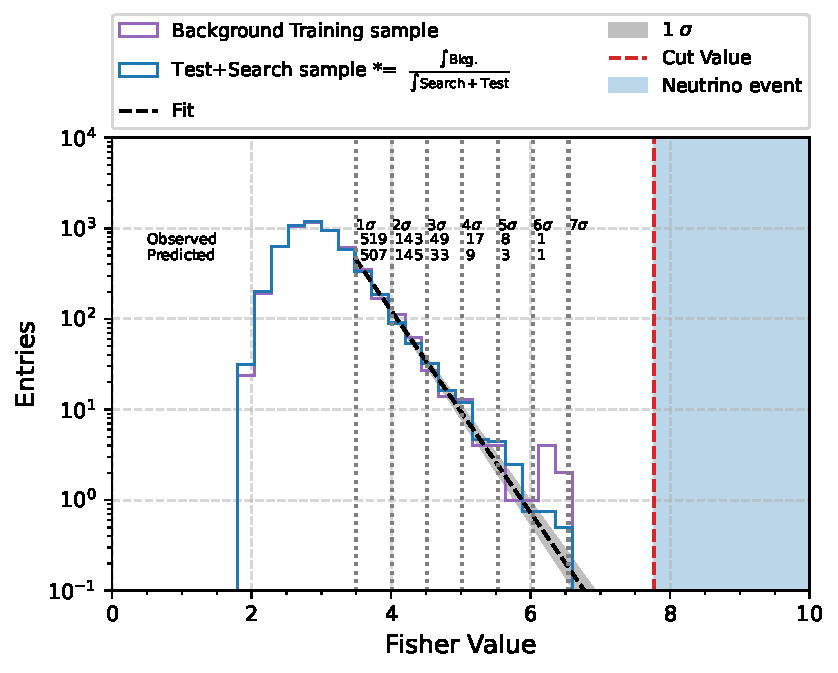
\includegraphics[width=\linewidth]{thesis_figures/Nu_analysis/Fisher_plots/Fisher_fit_search+test_bkg_region_58.5_61.5.pdf}
     \caption{$ 58.5^{\circ} <\theta_{\text{Rec}} \leq 61.5^{\circ}$}
     \label{fig:58.5-61.5}
   \end{subfigure}
   %\hfill
   \begin{subfigure}[r]{.48\textwidth}
     \centering
     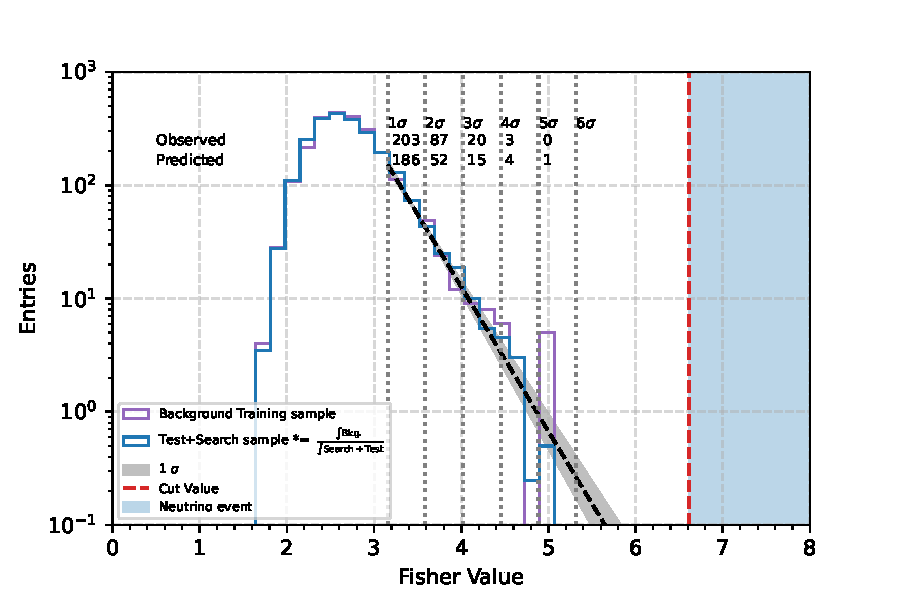
\includegraphics[width=\linewidth]{thesis_figures/Nu_analysis/Fisher_plots/Fisher_fit_search+test_bkg_region_61.5_64.5.pdf}
     \caption{$ 61.5^{\circ} <\theta_{\text{Rec}} \leq 64.5^{\circ}$}
    \end{subfigure}
    \hfill
    \begin{subfigure}[l]{.48\textwidth}
      \centering
      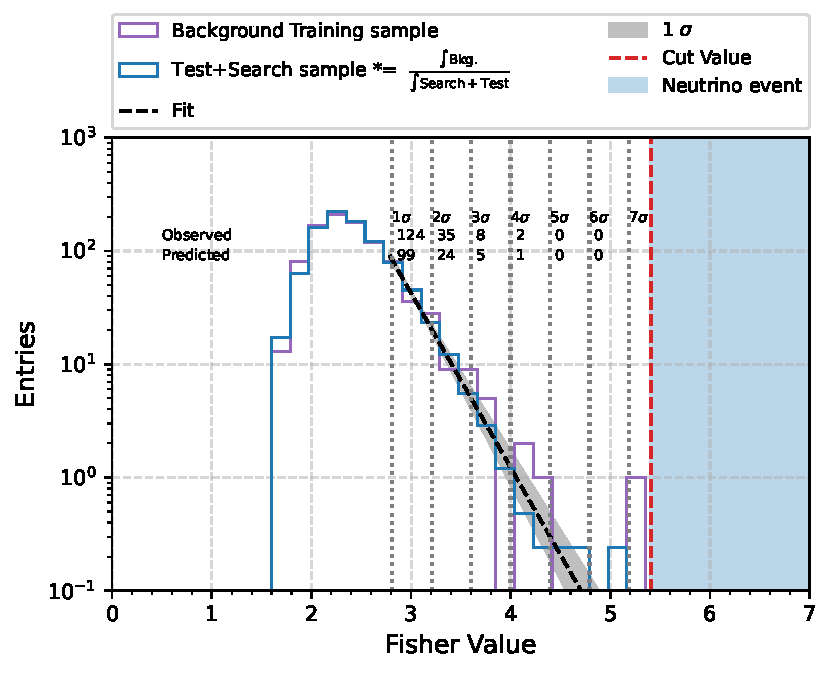
\includegraphics[width=\linewidth]{thesis_figures/Nu_analysis/Fisher_plots/Fisher_fit_search+test_bkg_region_64.5_67.5.pdf}
      \caption{$ 64.5^{\circ} <\theta_{\text{Rec}} \leq 67.5^{\circ}$}
    \end{subfigure}

    \begin{subfigure}[r]{.48\textwidth}
      \centering
      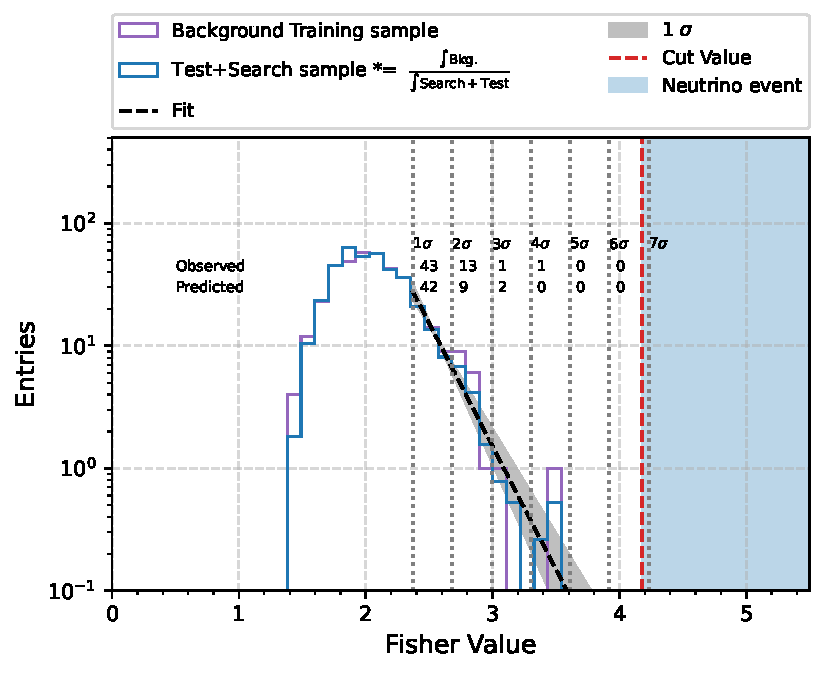
\includegraphics[width=\linewidth]{thesis_figures/Nu_analysis/Fisher_plots/Fisher_fit_search+test_bkg_region_67.5_70.5.pdf}
      \caption{$ 67.5^{\circ} <\theta_{\text{Rec}} \leq 70.5^{\circ}$}
    \end{subfigure}
    \hfill    
    \begin{subfigure}[r]{.48\textwidth}
      \centering
      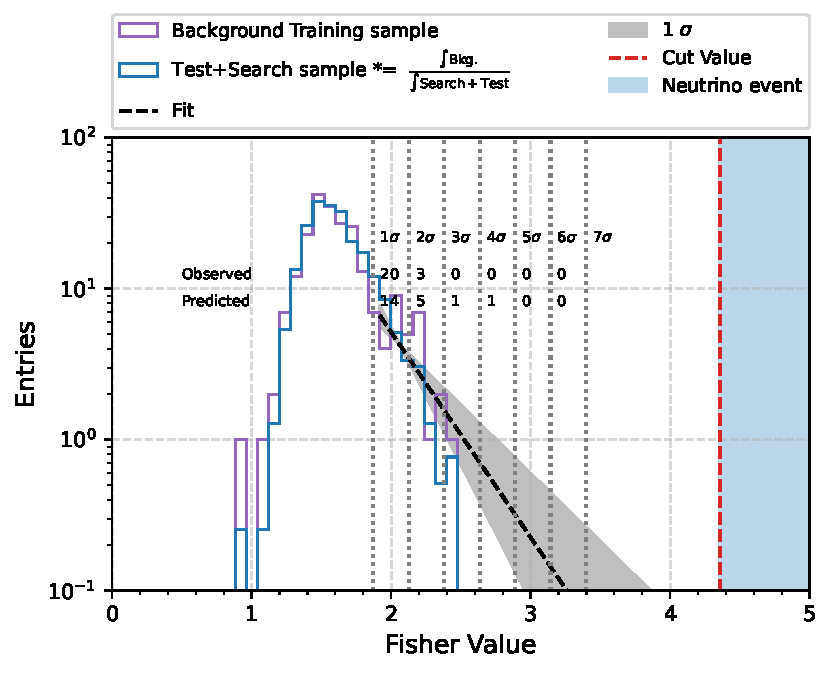
\includegraphics[width=\linewidth]{thesis_figures/Nu_analysis/Fisher_plots/Fisher_fit_search+test_bkg_region_70.5_73.5.pdf}
      \caption{$ 70.5^{\circ} <\theta_{\text{Rec}} \leq 76.5^{\circ}$}
   \end{subfigure}
   \caption{Comparison of the $\mathcal{F}$ value distributions for the background training (purple) and the test+search samples (blue) for the different angular sub-regions. The test+search sample is scaled by the ratio of the integrals of the background training and test+search samples. The black dashed line indicates the exponential fit to the tail of the distribution. The red dashed line indicates the value of the $\mathcal{F}_{\text{cut}}$ obtained from the fit. For the test+search sample the observed values are compared to the predicted values from the fit.}
    \label{fig:Fisher_cut_2}

\end{figure}
\FloatBarrier
\begin{table}[h!]
  \centering
  \small
  \begin{tabular}{ |P{1.25cm}||P{2.23cm}|P{2.23cm}|P{2.23cm}|P{2.23cm}|P{2.28cm}|  }
    \hline
      Fit & \multicolumn{5}{c|}{Number of events in $\mathcal{F}$ tails} \\
      Range & \multicolumn{5}{c|}{Observed - Predicted} \\
    \cline{2-6}
      & Region 1 & Region 2& Region 3& Region 4 & Region 5 \\
      &(58.5$^\circ$-61.5$^\circ$]&(61.5$^\circ$-64.5$^\circ$]&(64.5$^\circ$-67.5$^\circ$]& (67.5$^\circ$-70.5$^\circ$] & (70.5$^\circ$- 76.5$^\circ$] \\
    \hline 
    $\mu$ + 1$\sigma$ & 518.6 - 506.7 & 245.9 - 198.4 & 124.1 - 99.1 & 42.5 - 41.6 & 20.0 - 14.0 \\
    $\mu$ + 2$\sigma$ & 143.5 - 145.2 & 43.6 - 50.5 & 35.4 - 24.2 & 12.5 - 8.8 & 2.6 - 4.5 \\
    $\mu$ + 3$\sigma$ & 48.6 - 32.8 & 19.9 - 12.9 & 8.4 - 4.8 & 1.3 - 1.6 & 0.0 - 1.5 \\
    $\mu$ + 4$\sigma$ & 16.6 - 8.9 & 3.2 - 3.3 & 1.7 - 1.1 & 0.8 - 0.3 & 0.0 - 0.5 \\
    $\mu$ + 5$\sigma$ & 1.2 - 0.5 & 0.5 - 0.8 & 0.5 - 0.3 & 0.0 - 0.0 & 0.0 - 0.0 \\
    $\mu$ + 6$\sigma$ & 0.0 - 0.1 & 0.0 - 0.0 & 0.2 - 0.0 & 0.0 - 0.0 & 0.0 - 0.0 \\
    \hline
  \end{tabular}
  \caption{Evaluation of the exponential fit on the $\mathcal{F} $ distributions for test+search samples. The observed and predicted (from the fit) number of events in the tail of the Fisher distribution are shown for each angular sub-region. The numbers are calculated by integrating from the start point mentioned in the first row till the +1$\sigma$.}
  \label{tab:Cut_eval_unblind}
\end{table}

\section{Diffuse limit for the UHE neutrino flux}
\label{sec:diff_limit}
Since no neutrino candidate was found in this analysis, an upper limit to the flux of the incoming UHE$\nu$s can be estimated. Let flux per unit area, \textit{A}, energy, solid angle $\Omega$ and time be denoted by $\phi(E_{\nu}) = \frac{d^6 N_{\nu}}{dE_{\nu}\,d\Omega\, dA \, dt}$. The expected number of detected neutrinos can be calculated by folding in the total exposure $\xi_{tot}(E_{\nu})$ with flux as follows,

\begin{equation}
  N_{\text{expected}} = \int_{E_{\nu_{\text{min}}}}^{E_{\nu_{\text{max}}}} \phi(E_{\nu}) \cdot \xi_{\text{tot}}(E_{\nu}) \cdot dE_{\nu}
\end{equation}

Assuming a differential UHE$\nu$ flux $\phi = k \cdot E_{\nu}^{-2}$, the integrated upper limit on the value of k is given by:

\begin{equation}
  \label{eq:integ_lim}
  \mathrm{k_{up} = \frac{N_{up}}{\int_{E_{\nu min}}^{E_{\nu max}} E_{\nu}^{-2} \cdot \xi_{tot}(E_{\nu}) \cdot dE_{\nu}}} \, ,
\end{equation}

the value of $\mathrm{N_{up}}$ for a given confidence level can be determined based on the number of observed events and the number of expected background events. Different statistical methods can be used to obtain the value for $N_{up}$ based on the confidence interval. In the next sections some of these different statistical approaches are discussed in more detail. The Feldman and Cousins limit with an extension that incorporates the systematic uncertainties discussed above is chosen as a final estimate for $\mathrm{N_{up}}$.

\subsection{Feldman and Cousins limit}
\label{subsec:FandC}
Feldman-Cousins method~\cite{Feldman:1997qc} is a statistical technique used to construct confidence intervals, particularly for Poisson distributed data. This approach addressed the key shortcomings of traditional methods used to construct confidence intervals especially for cases where the number of observed events are low or zero. Traditional methods such as Gaussian approximation, which assume that data follows a normal distribution and are used to calculate confidence intervals can often lead to incorrect intervals particularly in rare event searches where the data is better described by a Poisson distribution. This can also lead to unphysical values e.g. negative value for rate of expected events. The Feldman-Cousins approach solves this problem by giving a unified method for constructing confidence intervals. The method ensures that the intervals are unbiased and do not favour one outcome over the other. It also ensures a natural transition from two-sided intervals (where there is significant data) to one-sided upper limits (when there is little to no data). The method also respects physical constraints, such as non-negative values for expected event rates. It also provides intervals with more accurate coverage probabilities, reducing over-coverage issues common in other methods. 

The Feldman \& Cousins approach is implemented as a part of \textit{gammapy} in python~\cite{Gammapy:2023gvb} which was used to get the interval for this analysis. The information was also verified with look-up tables in~\cite{Feldman:1997qc}. For a 90\% confidence interval, in case of zero signal and background events, the upper and lower limits are given as $N^{90\%}_{\text{up}} = 2.44$ and $N^{90\%}_{\text{\text{low}}} = 0$ respectively. If one signal event is seen with zero background then this interval shifts to [4.36, 0.11]. It is important to note that both statistical and systematic uncertainties are not included for the intervals calculated in the Feldman \& Cousins method. 

\subsection{Rolke approach}
\label{subsec:Rolke}
The Feldman \& Cousins treatment is a frequentist method which requires the background source to be known precisely. Such a method can fail if the uncertainties are too high~\cite{Rolke:2000ij}. To solve this problem one can also use the Rolke method~\cite{Rolke:2004mj} which incorporates prior information in this case signal with a Poisson distribution and background with either a Poisson or Gaussian distribution. The method is implemented as a ROOT class under TRolke~\cite{TRolke_ROOT}. For a 90\% confidence interval in the case of zero signal and background events the interval is given as [2.21, 0] assuming a Poisson distribution for both signal and background. As it is seen the interval is smaller in comparison to the Feldman \& Cousins approach. This can be explained much more clearly for the case where there is one signal event and no background where the Rolke interval is [3.65,0]. In this case according to the Feldman \& Cousins approach the event has to be a signal since the lower limit is > 0 but in the Rolke approach it is still possible that such an event in the signal region could be a background event i.e. in the Rolke approach the absence of background does not imply zero background, but it only means that the background is not too large. This is because the background is treated as a Poisson number. Thus, the overall upper and lower limits in the Rolke approach are always smaller in comparison to the Feldman \& Cousins  method. 

\subsection{Conrad approach}
\label{subsec:Conrad}
The Conrad method for calculating confidence intervals allows the inclusion of systematic uncertainties in the evaluation. Using this approach the uncertainties in the background prediction, background detection and the signal detection efficiencies can be incorporated in the confidence interval calculation by integrating over the PDFs of these parameters~\cite{Conrad:2002kn}. The method computes the upper limit based on a likelihood ratio between the observed data and the null hypothesis (no signal). For this work the interval was calculated using POLE++~\cite{Conrad:2005zm} which is a C++ program that implements the Conrad method. The systematic uncertainty on exposure was estimated to be as [+20\%, -14\%] as mentioned in section~\ref{sec:det_uncert}. Using a uniform PDF to characterize the exposure and a Gaussian assumption for background, for a 90\% confidence interval in the case of zero signal and background events the upper and lower limits are given as: 

\begin{equation}
  \label{eq:Conrad_lim}
  N^{90\%}_{up} = 2.39, \,N^{90\%}_{\text{low}} = 0
\end{equation}

The interval is smaller in comparison to the Feldman \& Cousins method due to the uneven interval for the systematic uncertainty. 

\subsection{Final calculation}
\label{subsec:final_lim}
After the determination of $N_{\text{up}}$ using the Conrad approach the equation~\ref{eq:integ_lim} can be solved to determine the upper limit to the diffused flux of UHE$\nu$s. The integral goes from $E_{\text{min}} = 10^{17.5} $eV till $E_{\text{max}} = 10^{20.5} $eV which is the total energy range explored in the simulations. It is also important to note that the limit is only valid for a smaller energy window. The single flavour 90\% C.L. integrated limit is given by 
\begin{equation}
  \label{eq:final_lim} 
  \mathrm{k_{90} < 1.9 x 10^{-7} GeV cm^{-2} s^{-1} sr^{-1}}.
\end{equation}
It applies to an energy range of $E_{\nu} \epsilon [1.3 \times 10^{18} - 2.5 \times 10^{19.5}]$ which is the energy range for which $\sim$90\% total event rate is expected in the case of $E^{-2}_{\nu}$ flux. The value along with the 90\% energy range is plotted as a dashed purple line in Fig.~\ref{fig:Limit_comp_1}.

\begin{figure}[t!]
  \centering
  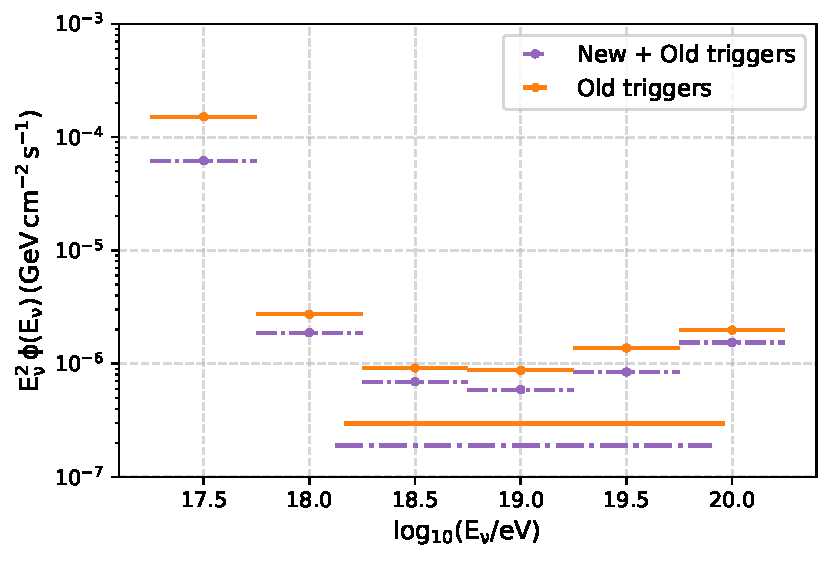
\includegraphics[width=14.5cm]{thesis_figures/ExpLimits/Integ_DiffLimit_comp_new_sim_optim.pdf}
  \caption{Integral (90\% C.L., long purple dashed lines) and differential upper limits (short purple segments) for the UHE$\nu$s diffuse flux in the DG$\mathrm{_{\text{low}}}$ region. The limits for an analysis without the new triggers are also plotted in orange for comparison. Both the limits are calculated for the time period 2014-2021.}
  \label{fig:Limit_comp_1}
\end{figure}

The other dashed purple lines with central dots are the \textit{differential limits}. These are calculated by integrating the denominator of eq.~\ref{eq:integ_lim} in bins of width $\Delta = 0.5eV$ in $\log_{10}(E_{\nu})$. Mathematically for the $i^{th}$ bin this can be represented as follows:

\begin{equation}
  \label{eq:diff_lim}
  \text{Differential limit} \, (i^{\text{th}} \, E_{\nu} \, \text{bin})  = \frac{N_{\text{Up}}}{\int_{\log_{10}(E^i - (\Delta \log_{10}E)/2)}^{\log_{10}(E^i + (\Delta \log_{10}E)/2)} E^{-1}_{\nu} \cdot \xi(E_{\nu}) \cdot ln(10) \cdot d(\log_{10}(E_{\nu}))}
\end{equation}

Assuming constant exposure and flux in each energy bin the differential limit can be estimated as:

\begin{equation}
  \label{eq:diff_lim_approx}
 \text{Approx. Differential limit} \, (i^{\text{th}} \, E_{\nu} \, \text{bin})  = \frac{N_{\text{Up}}}{E^{-1}_{\nu} \cdot \xi(E_{\nu}) \cdot ln(10) \cdot \Delta (\log_{10}(E_{\nu}))}
\end{equation}
\begin{figure}[t!]
  \centering
  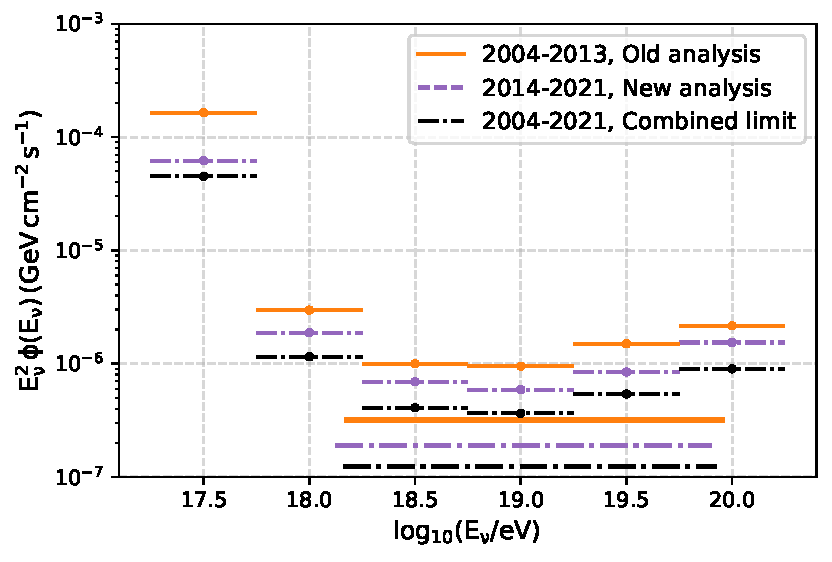
\includegraphics[width=14.5cm]{thesis_figures/ExpLimits/Integ_DiffLimit_comp_combined_new_sim_optim.pdf}
  \caption{Combination of Integral and differential upper limits for a UHE$\nu$s diffuse flux in the angular range, $ 58.5^{\circ} <\theta_{\text{Rec}} \leq 61.5^{\circ}$, for the time period 2004-2021. The limits for the time period 2004-2013 are plotted in orange and the limits for the time period 2014-2021 are plotted in purple. The combined limits are plotted in black.}
  \label{fig:Limit_comp_2}
\end{figure}

These limits provide a way to denote the sensitivity of the detector for different energies. As it can be seen from the Fig.~\ref{fig:Limit_comp_1} for the Down-going Low analysis the Pierre Auger Observatory is the most sensitive for energies $\sim$1 EeV. 

Both limits are also compared to the results from the previous analysis in Fig.~\ref{fig:Limit_comp_1}. As it was seen in the exposure comparison it is clear that the new triggers help improve the sensitivity at lower energies. For higher energies the improvements to the upper-limit for the diffuse flux of UHE${\nu}$s though not as significant is still substantial. This improvement can be attributed to the changes in the Fisher analysis. The integral flux limit sees an improvement of $\sim$ 40\%. 

Furthermore, the limits obtained in this analysis are combined with the limits obtained using the old analysis. The total exposure for the time period 2004-2013 is calculated using the old analysis and selection as ToTd and MoPS were not implemented for this time period. This exposure is combined with the exposure obtained in this study with the inclusion of new triggers for the time period 2014-2021. This combination is only done under the assumption that the systematics for both the analysis are very similar. The combined exposure is then used to calculate the overall differential and integral limits for the DG$_{\text{\text{low}}}$ region in the time period 2004-2021. This is shown in Fig.~\ref{fig:Limit_comp_2}. Further this combination is also compared to the expected limit if only the old analysis is applied to the time period 2004-2021. This is shown in Fig.~\ref{fig:Limit_comp_3}.



\begin{figure}[h!]
  \centering
  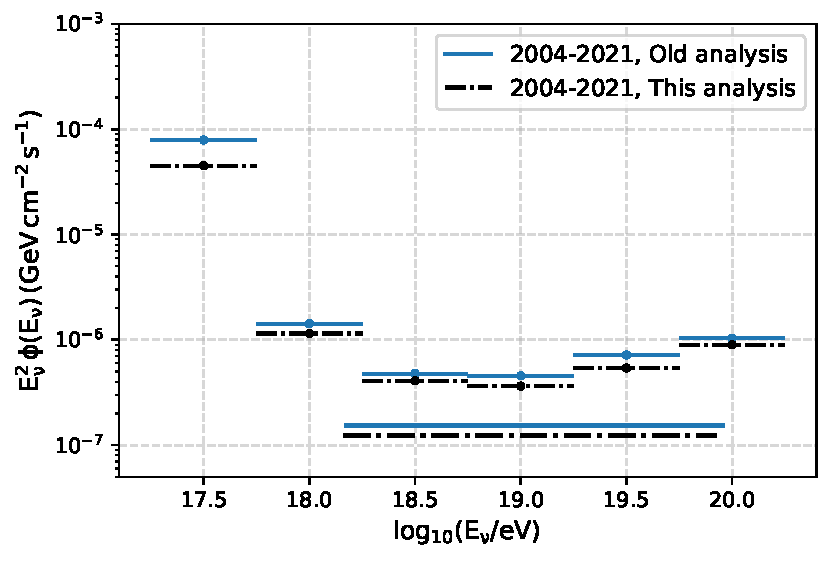
\includegraphics[width=14.5cm]{thesis_figures/ExpLimits/Integ_DiffLimit_comp_combined_new_sim_optim_3.pdf}
  \caption{Comparison of the combined limits to the expected limits if only the old analysis is applied to the time period 2004-2021. The limits obtained in this study are plotted in black while the limits obtained from the old analysis for the same time period are plotted in blue.}
  \label{fig:Limit_comp_3}
\end{figure}

The diffuse flux limit and sensitivity for Auger is dominated by the Earth-skimming channel as shown in~\cite{Aab_2019_diffuse}. This limit is significantly lower than the DG$\mathrm{_{\text{low}}}$ channel and is the main driver to constrain astrophysical and cosmogenic models. A comparison of the limits obtained in this study to the overall limit set at the Pierre Auger Observatory along with the flux predictions from some popular cosmogenic and astrophysical models is shown in Fig.~\ref{fig:Limit_comp_overall}. The aim of this study was to evaluate the improvement, but it was always known that unless huge, the inclusion of new triggers does not improve the overall diffuse flux limits set using the data collected by the Pierre Auger Observatory. However, the improvements shown in this analysis are more important in the context of point source searches. This is discussed more in the next chapter. 

\begin{figure}[h!]
  \centering
  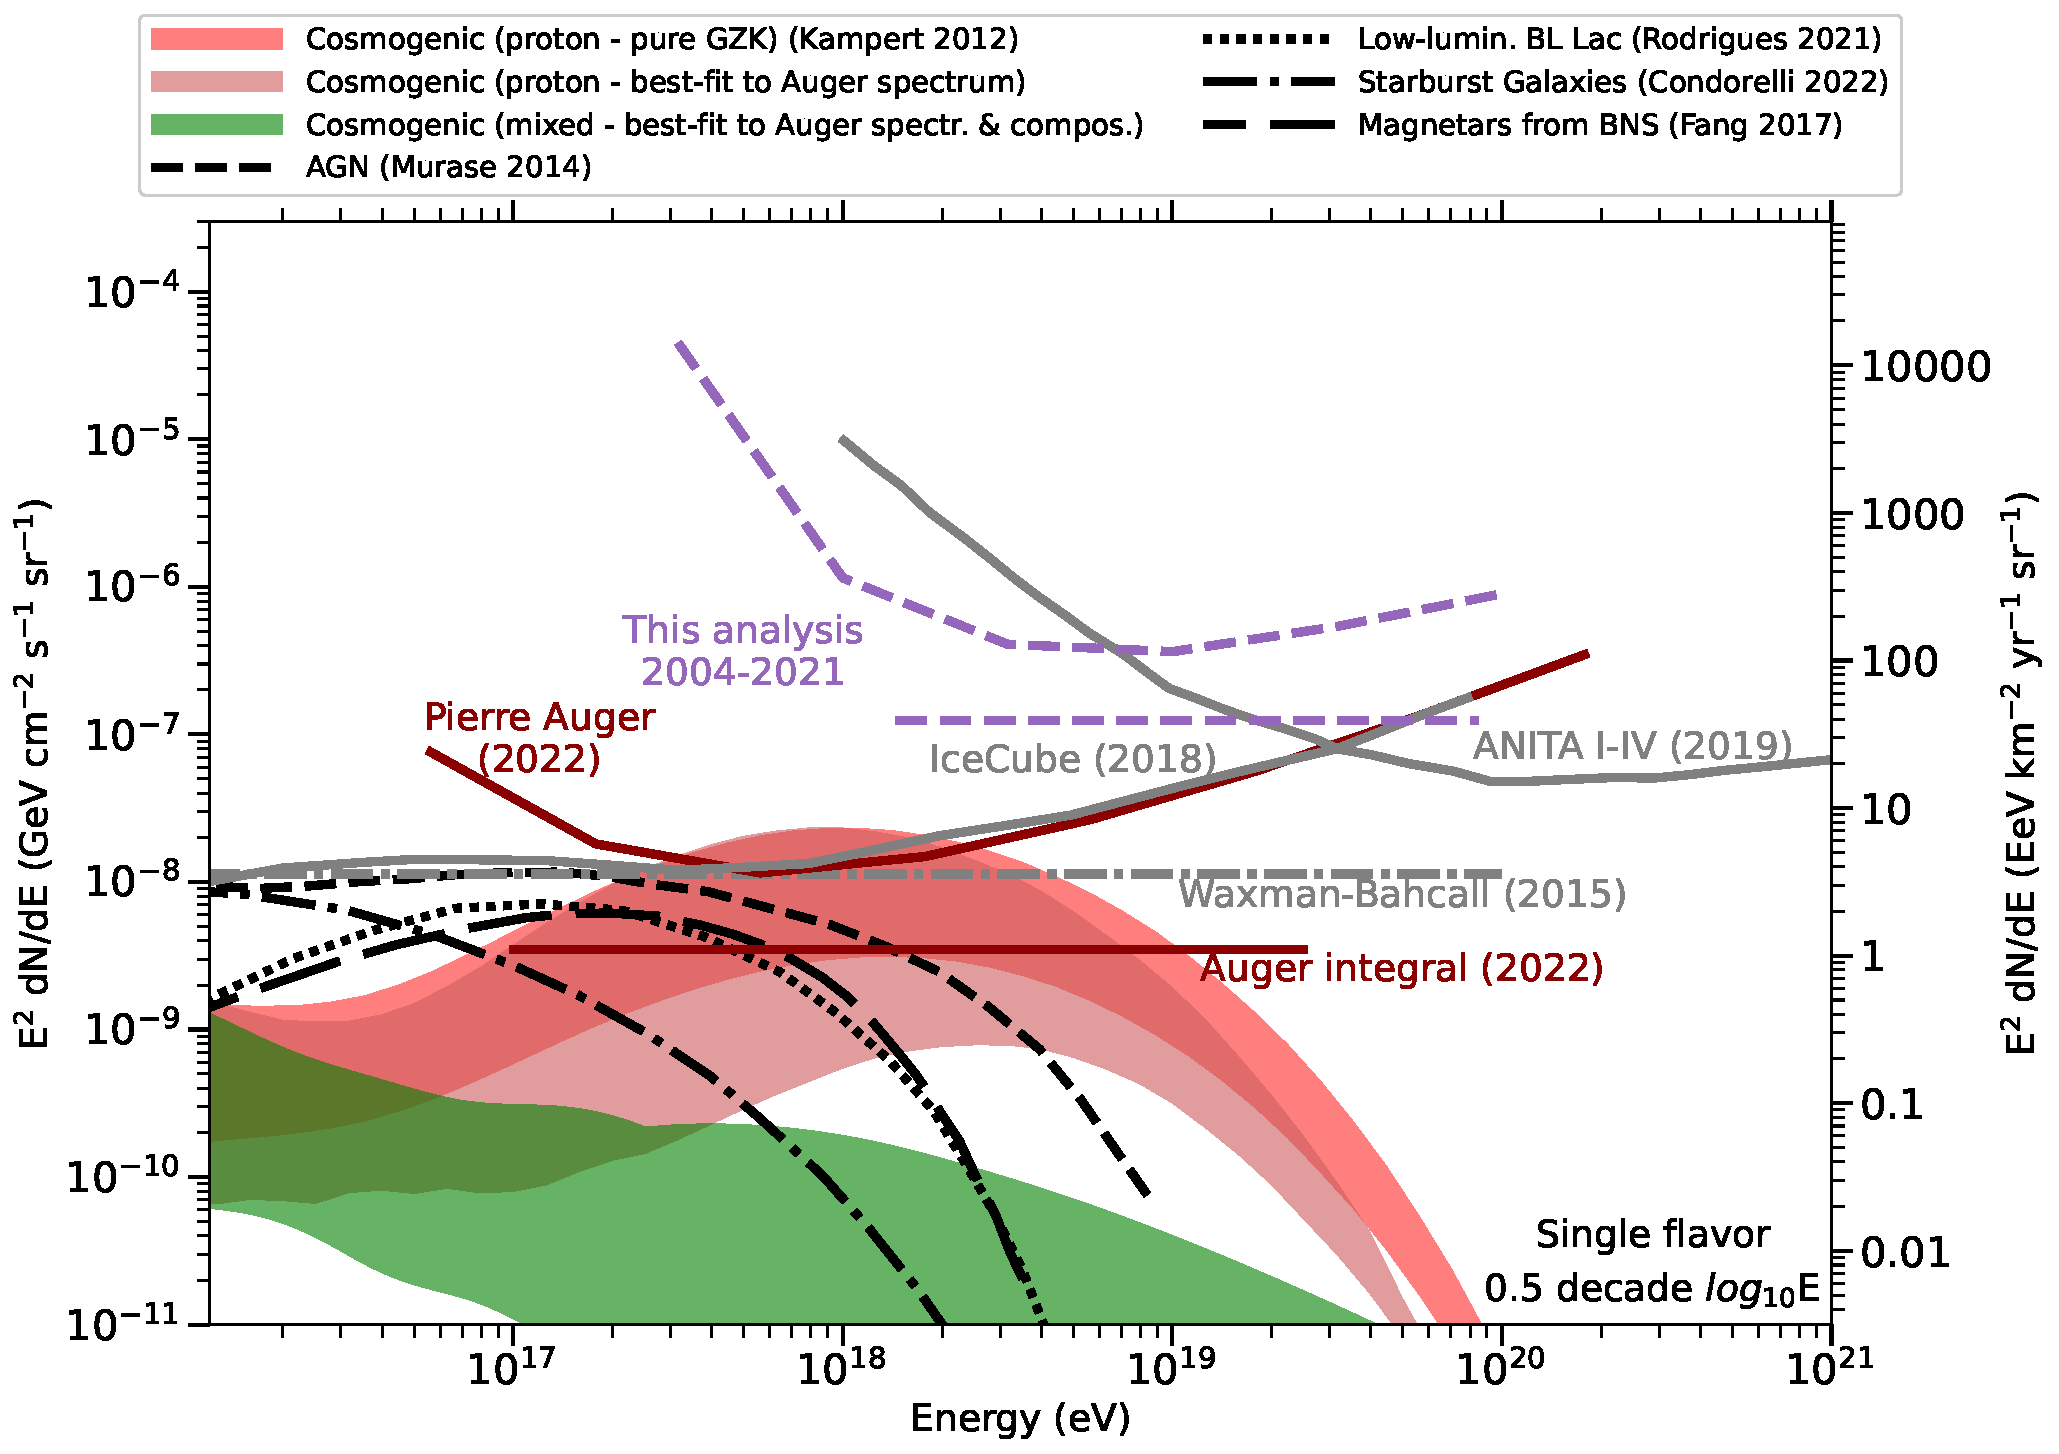
\includegraphics[width=14.5cm]{thesis_figures/ExpLimits/limits_and_models_DGL.pdf}
  \caption{Comparison of the combined limits obtained in this analysis to the current upper limits on the diffuse flux of cosmogenic neutrinos. The predicted fluxes from a few cosmogenic and astrophysical models is also shown for comparison. The plot has been modified to add the limits of this analysis using code provided by J. Muñiz and is originally taken from ~\cite{PierreAuger:2023pjg}}
  \label{fig:Limit_comp_overall}
\end{figure}



%%% Local Variables:
%%% mode: latex
%%% TeX-master: "mythesis"
%%% End:
